%% ****** Start of file apstemplate.tex ****** %
%%
%%
%%   This file is part of the APS files in the REVTeX 4 distribution.
%%   Version 4.1r of REVTeX, August 2010
%%
%%
%%   Copyright (c) 2001, 2009, 2010 The American Physical Society.
%%
%%   See the REVTeX 4 README file for restrictions and more information.
%%
%
% This is a template for producing manuscripts for use with REVTEX 4.0
% Copy this file to another name and then work on that file.
% That way, you always have this original template file to use.
%
% Group addresses by affiliation; use superscriptaddress for long
% author lists, or if there are many overlapping affiliations.
% For Phys. Rev. appearance, change preprint to twocolumn.
% Choose pra, prb, prc, prd, pre, prl, prstab, prstper, or rmp for journal
%  Add 'draft' option to mark overfull boxes with black boxes
%  Add 'showpacs' option to make PACS codes appear
%  Add 'showkeys' option to make keywords appear
\documentclass[aps,pre,preprint,groupedaddress, twocolumn, floatfix]{revtex4-1}
\input ../inputs/setupSveZha
\input ../inputs/editsDasbuch   %% editing comments, DasBuch style
\input ../inputs/def            %% do not edit; update from dasbuch/book/inputs/def.tex
\input ../inputs/defsSveZha     %% all diffusion project edits: \renewcommand, etc
\usepackage[pdftex]{graphicx}
\graphicspath{{../figs/}{../tingnan/figs/}{../Fig/}{ChaosBook/}}  %% directories with graphics
%\documentclass[aps,prl,preprint,superscriptaddress]{revtex4-1}
%\documentclass[aps,prl,reprint,groupedaddress]{revtex4-1}

% You should use BibTeX and apsrev.bst for references
% Choosing a journal automatically selects the correct APS
% BibTeX style file (bst file), so only uncomment the line
% below if necessary.
%\bibliographystyle{apsrev4-1}

\begin{document}

% Use the \preprint command to place your local institutional report
% number in the upper righthand corner of the title page in preprint mode.
% Multiple \preprint commands are allowed.
% Use the 'preprintnumbers' class option to override journal defaults
% to display numbers if necessary
%\preprint{}

%Title of paper
\title{Diffuse globally, compute locally: a cyclist tale}

% repeat the \author .. \affiliation  etc. as needed
% \email, \thanks, \homepage, \altaffiliation all apply to the current
% author. Explanatory text should go in the []'s, actual e-mail
% address or url should go in the {}'s for \email and \homepage.
% Please use the appropriate macro foreach each type of information

% \affiliation command applies to all authors since the last
% \affiliation command. The \affiliation command should follow the
% other information
% \affiliation can be followed by \email, \homepage, \thanks as well.
\author{Tingnan Zhang, Daniel I. Goldman and Predrag Cvitanovi\'c}
\email[corresponding to: ]{predrag@gatech.edu}
%\homepage[]{Your web page}
%\thanks{}
%\altaffiliation{}
\affiliation{School of Physics, Georgia Institute of Technology}

%Collaboration name if desired (requires use of superscriptaddress
%option in \documentclass). \noaffiliation is required (may also be
%used with the \author command).
%\collaboration can be followed by \email, \homepage, \thanks as well.
%\collaboration{}
%\noaffiliation

\date{\today}

\begin{abstract}
The 2-dimensional Lorentz gas models the diffusive motion of a light
molecule within a large number of heavy scatters by a point particle
bouncing off a collection of reflecting disks in a plane. Proposed by H.
A. Lorentz at 1905, the model has been not only useful in studying dilute
electron gas thermal and diffusive properties (in approximation where
electron-electron interactions are ignored), but also in dynamical
systems/statistical physics to answer fundamental questions on how
ergodicity arises from determinism. Motivated by a recent potential
application to macroscopic transport (statistics of robotic locomotion
paths over a heterogeneous terrain strewn with scatterers), we present a
very precise computation (not a numerical simulation, but an evaluation
of the exact periodic orbit theory formula for the diffusion constant)
for a periodic triangular Lorentz gas with finite horizon. We formulate a
new approach to tiling the plane in terms of three elementary tiling
generators which, for the first time, enables us to use periodic orbits
computed in the fundamental domain (that is, $1/12$ of the hexagonal
elementary cell whose translations tile the entire plane). Compared with
previous literature (which, amusingly, explicitly states that our
calculation cannot be done), our fundamental domain value of the
diffusion constant converges quickly for inter-disk separation/disk
radius $>0.2$, with the cycle expansion truncated to only a few hundred
periodic orbits of up to $5$ billiard wall bounces. For small inter-disk
separations, with periodic orbits up to $6$ bounces, our diffusion
constants are close ($<10\%$) to direct numerical simulation estimates,
as well as the recent literature probabilistic estimates.
\end{abstract}
% insert suggested PACS numbers in braces on next line
\pacs{}
% insert suggested keywords - APS authors don't need to do this
%\keywords{}

%\maketitle must follow title, authors, abstract, \pacs, and \keywords
\maketitle

% body of paper here - Use proper section commands
% References should be done using the \cite, \ref, and \label commands

\section{Introduction}
\begin{figure}[htbp]
\begin{center}
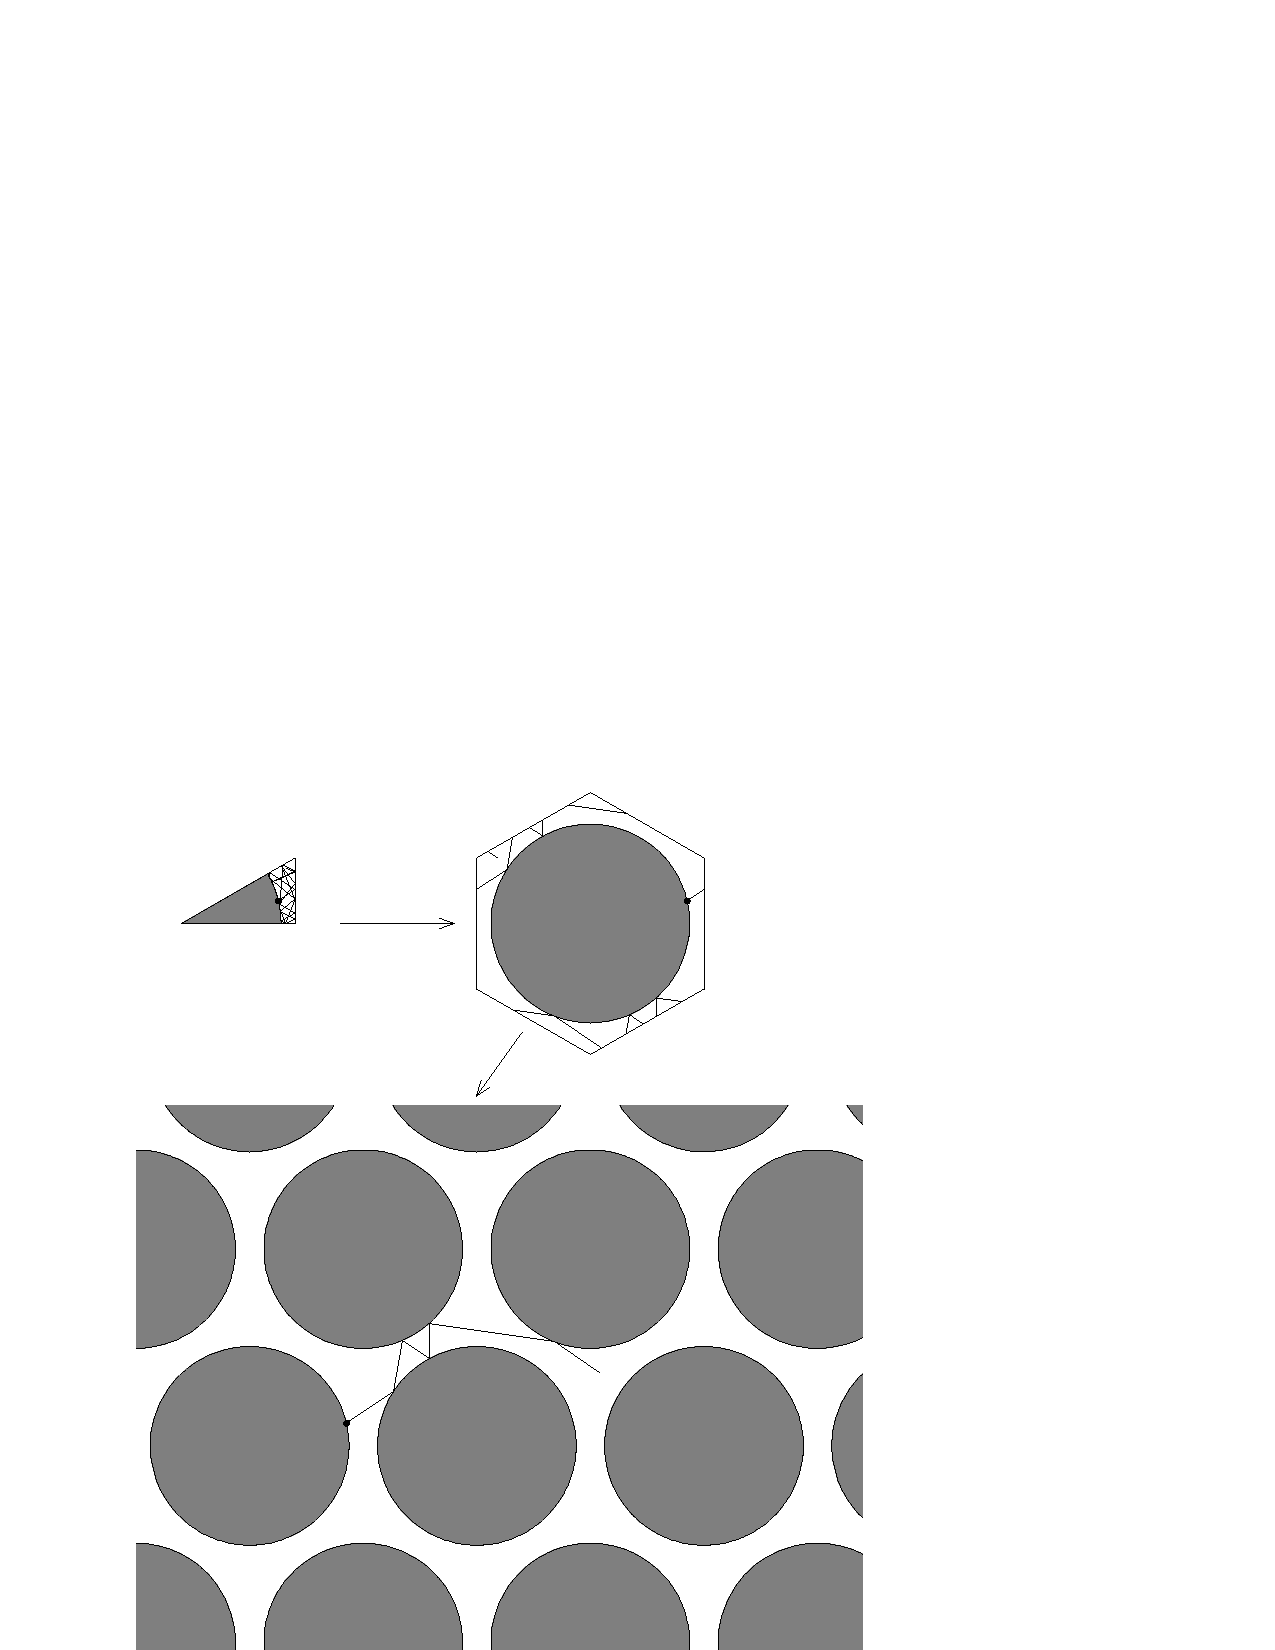
\includegraphics[width=0.45\textwidth]{schreiberFig1}
\caption[]{Motion in Fundamental Domain (FD), Elementary Cell (EC) and full space. \label{fig:schrieberFig1}}
\end{center}
\end{figure}
\begin{figure}[htbp]
\begin{center}
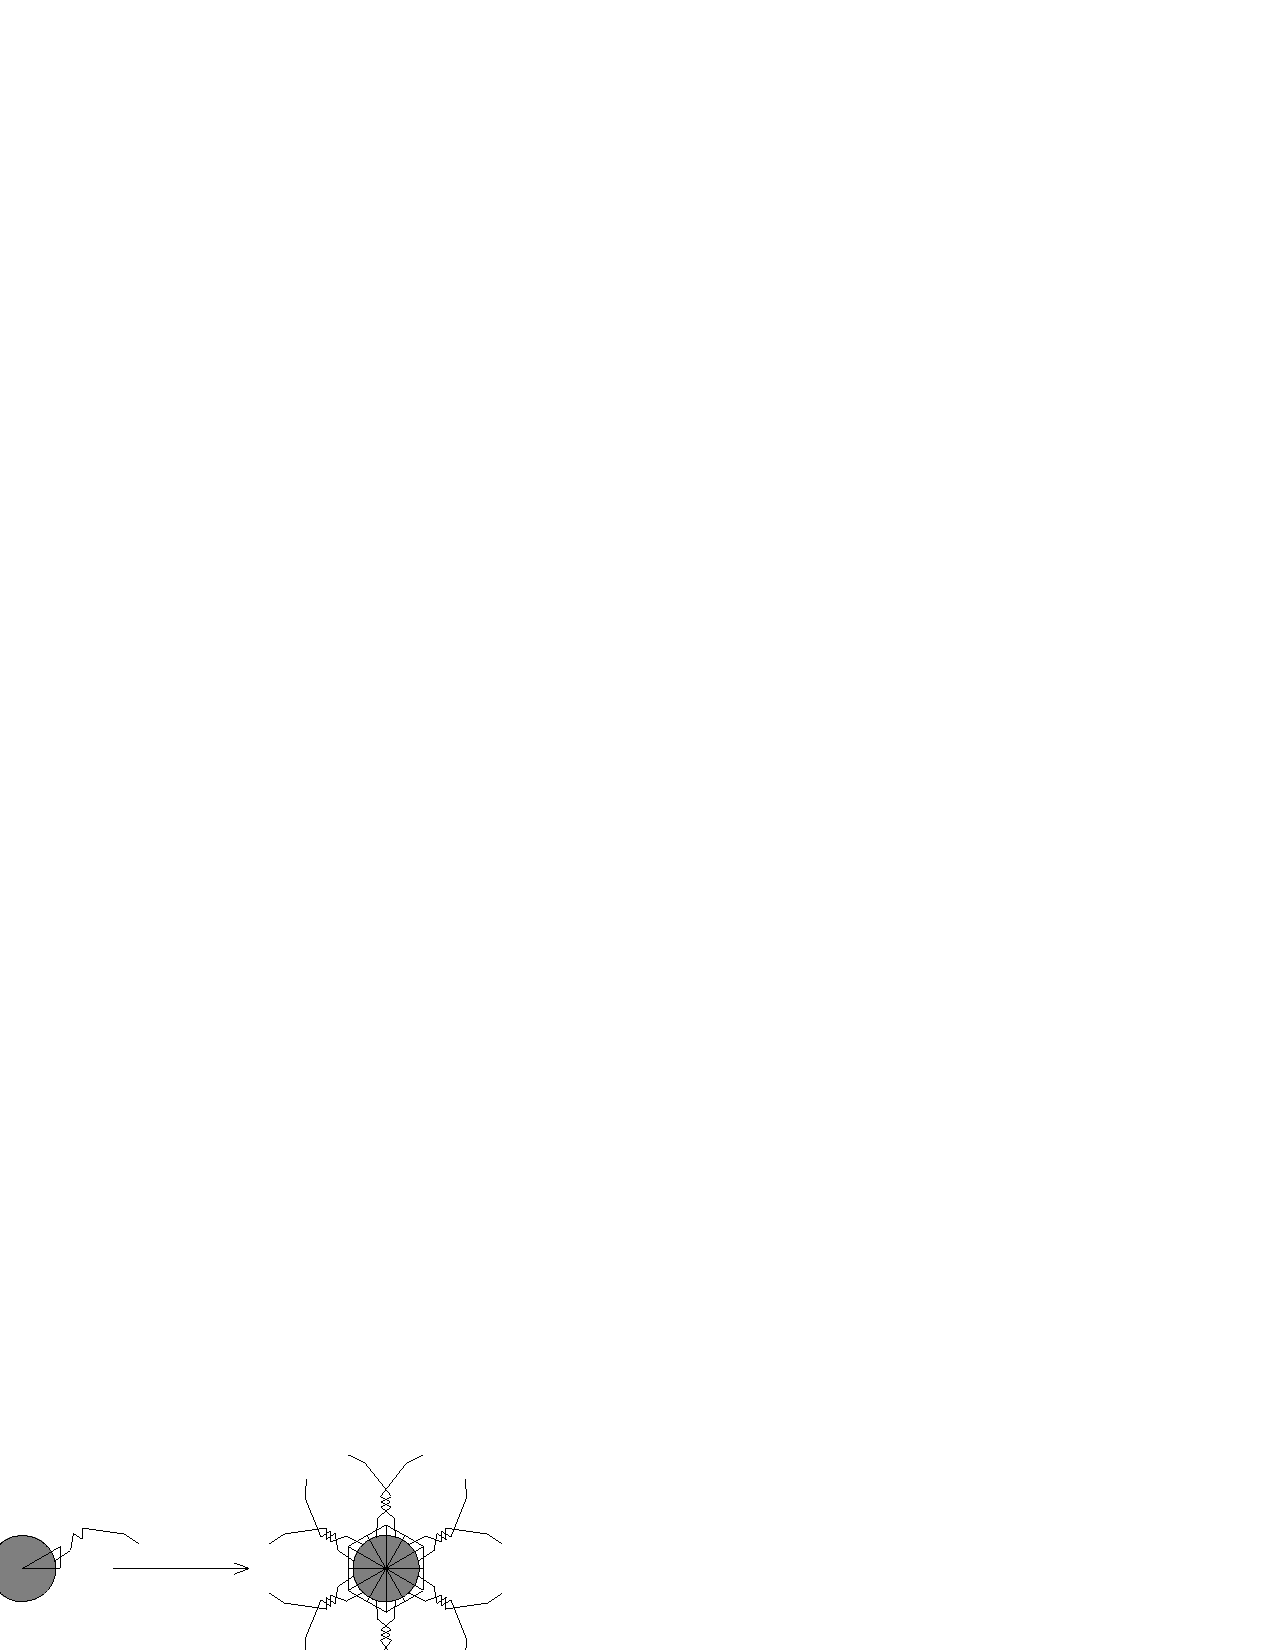
\includegraphics[width=0.45\textwidth]{schreiberFig2}
\caption[]{An (unwrapped) trajectory (in full space) and its 12 copies after applying point group actions to it. \label{fig:schrieberFig2}}
\end{center}
\end{figure}
\begin{figure}[htbp]
\begin{center}
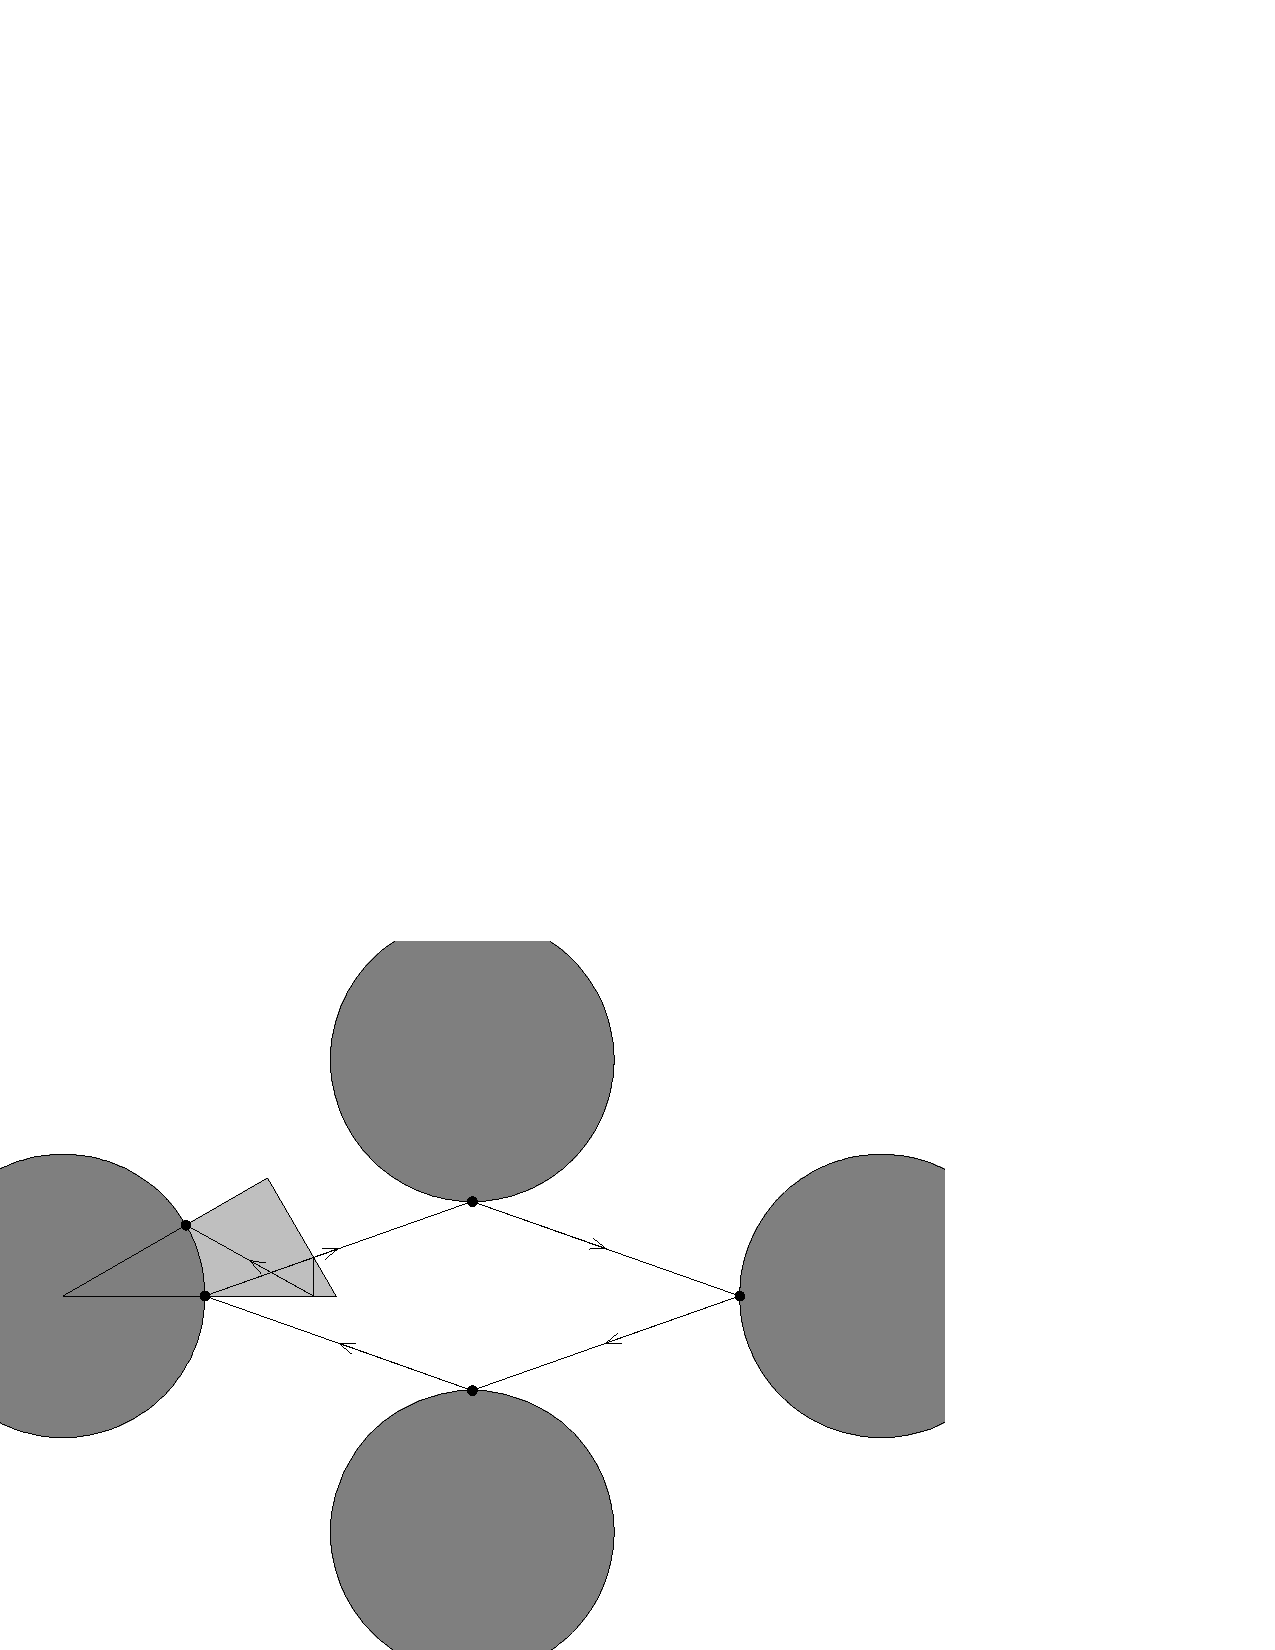
\includegraphics[width=0.45\textwidth]{schreiberFig3}
\caption[]{Multiplicity of periodic orbits in FD. \label{fig:schrieberFig3}}
\end{center}
\end{figure}
\section{Diffusion Confusion}

\section{Results and Discussions}

% Put \label in argument of \section for cross-referencing
%\section{\label{}}

% If in two-column mode, this environment will change to single-column
% format so that long equations can be displayed. Use
% sparingly.
%\begin{widetext}
% put long equation here
%\end{widetext}

% figures should be put into the text as floats.
% Use the graphics or graphicx packages (distributed with LaTeX2e)
% and the \includegraphics macro defined in those packages.
% See the LaTeX Graphics Companion by Michel Goosens, Sebastian Rahtz,
% and Frank Mittelbach for instance.
%
% Here is an example of the general form of a figure:
% Fill in the caption in the braces of the \caption{} command. Put the label
% that you will use with \ref{} command in the braces of the \label{} command.
% Use the figure* environment if the figure should span across the
% entire page. There is no need to do explicit centering.

% \begin{figure}
% \includegraphics{}%
% \caption{\label{}}
% \end{figure}

% Surround figure environment with turnpage environment for landscape
% figure
% \begin{turnpage}
% \begin{figure}
% \includegraphics{}%
% \caption{\label{}}
% \end{figure}
% \end{turnpage}

% tables should appear as floats within the text
%
% Here is an example of the general form of a table:
% Fill in the caption in the braces of the \caption{} command. Put the label
% that you will use with \ref{} command in the braces of the \label{} command.
% Insert the column specifiers (l, r, c, d, etc.) in the empty braces of the
% \begin{tabular}{} command.
% The ruledtabular enviroment adds doubled rules to table and sets a
% reasonable default table settings.
% Use the table* environment to get a full-width table in two-column
% Add \usepackage{longtable} and the longtable (or longtable*}
% environment for nicely formatted long tables. Or use the the [H]
% placement option to break a long table (with less control than 
% in longtable).
% \begin{table}%[H] add [H] placement to break table across pages
% \caption{\label{}}
% \begin{ruledtabular}
% \begin{tabular}{}
% Lines of table here ending with \\
% \end{tabular}
% \end{ruledtabular}
% \end{table}

% Surround table environment with turnpage environment for landscape
% table
% \begin{turnpage}
% \begin{table}
% \caption{\label{}}
% \begin{ruledtabular}
% \begin{tabular}{}
% \end{tabular}
% \end{ruledtabular}
% \end{table}
% \end{turnpage}

% Specify following sections are appendices. Use \appendix* if there
% only one appendix.
%\appendix
%\section{}

% If you have acknowledgments, this puts in the proper section head.
%\begin{acknowledgments}
% put your acknowledgments here.
%\end{acknowledgments}

% Create the reference section using BibTeX:
\bibliography{../bibtex/siminos}

\end{document}
%
% ****** End of file apstemplate.tex ******

